
%% bare_conf.tex
%% V1.3
%% 2007/01/11
%% by Michael Shell
%% See:
%% http://www.michaelshell.org/
%% for current contact information.
%%
%% This is a skeleton file demonstrating the use of IEEEtran.cls
%% (requires IEEEtran.cls version 1.7 or later) with an IEEE conference paper.
%%
%% Support sites:
%% http://www.michaelshell.org/tex/ieeetran/
%% http://www.ctan.org/tex-archive/macros/latex/contrib/IEEEtran/
%% and
%% http://www.ieee.org/

%%*************************************************************************
%% Legal Notice:
%% This code is offered as-is without any warranty either expressed or
%% implied; without even the implied warranty of MERCHANTABILITY or
%% FITNESS FOR A PARTICULAR PURPOSE! 
%% User assumes all risk.
%% In no event shall IEEE or any contributor to this code be liable for
%% any damages or losses, including, but not limited to, incidental,
%% consequential, or any other damages, resulting from the use or misuse
%% of any information contained here.
%%
%% All comments are the opinions of their respective authors and are not
%% necessarily endorsed by the IEEE.
%%
%% This work is distributed under the LaTeX Project Public License (LPPL)
%% ( http://www.latex-project.org/ ) version 1.3, and may be freely used,
%% distributed and modified. A copy of the LPPL, version 1.3, is included
%% in the base LaTeX documentation of all distributions of LaTeX released
%% 2003/12/01 or later.
%% Retain all contribution notices and credits.
%% ** Modified files should be clearly indicated as such, including  **
%% ** renaming them and changing author support contact information. **
%%
%% File list of work: IEEEtran.cls, IEEEtran_HOWTO.pdf, bare_adv.tex,
%%                    bare_conf.tex, bare_jrnl.tex, bare_jrnl_compsoc.tex
%%*************************************************************************

% *** Authors should verify (and, if needed, correct) their LaTeX system  ***
% *** with the testflow diagnostic prior to trusting their LaTeX platform ***
% *** with production work. IEEE's font choices can trigger bugs that do  ***
% *** not appear when using other class files.                            ***
% The testflow support page is at:
% http://www.michaelshell.org/tex/testflow/



% Note that the a4paper option is mainly intended so that authors in
% countries using A4 can easily print to A4 and see how their papers will
% look in print - the typesetting of the document will not typically be
% affected with changes in paper size (but the bottom and side margins will).
% Use the testflow package mentioned above to verify correct handling of
% both paper sizes by the user's LaTeX system.
%
% Also note that the "draftcls" or "draftclsnofoot", not "draft", option
% should be used if it is desired that the figures are to be displayed in
% draft mode.
%
\documentclass[conference]{IEEEtran}
% Add the compsoc option for Computer Society conferences.
%
% If IEEEtran.cls has not been installed into the LaTeX system files,
% manually specify the path to it like:
% \documentclass[conference]{../sty/IEEEtran}





% Some very useful LaTeX packages include:
% (uncomment the ones you want to load)


% *** MISC UTILITY PACKAGES ***
%
%\usepackage{ifpdf}
% Heiko Oberdiek's ifpdf.sty is very useful if you need conditional
% compilation based on whether the output is pdf or dvi.
% usage:
% \ifpdf
%   % pdf code
% \else
%   % dvi code
% \fi
% The latest version of ifpdf.sty can be obtained from:
% http://www.ctan.org/tex-archive/macros/latex/contrib/oberdiek/
% Also, note that IEEEtran.cls V1.7 and later provides a builtin
% \ifCLASSINFOpdf conditional that works the same way.
% When switching from latex to pdflatex and vice-versa, the compiler may
% have to be run twice to clear warning/error messages.






% *** CITATION PACKAGES ***
%
%\usepackage{cite}
% cite.sty was written by Donald Arseneau
% V1.6 and later of IEEEtran pre-defines the format of the cite.sty package
% \cite{} output to follow that of IEEE. Loading the cite package will
% result in citation numbers being automatically sorted and properly
% "compressed/ranged". e.g., [1], [9], [2], [7], [5], [6] without using
% cite.sty will become [1], [2], [5]--[7], [9] using cite.sty. cite.sty's
% \cite will automatically add leading space, if needed. Use cite.sty's
% noadjust option (cite.sty V3.8 and later) if you want to turn this off.
% cite.sty is already installed on most LaTeX systems. Be sure and use
% version 4.0 (2003-05-27) and later if using hyperref.sty. cite.sty does
% not currently provide for hyperlinked citations.
% The latest version can be obtained at:
% http://www.ctan.org/tex-archive/macros/latex/contrib/cite/
% The documentation is contained in the cite.sty file itself.






% *** GRAPHICS RELATED PACKAGES ***
%
\ifCLASSINFOpdf
  \usepackage[pdftex]{graphicx}
  % declare the path(s) where your graphic files are
  % \graphicspath{{../pdf/}{../jpeg/}}
  % and their extensions so you won't have to specify these with
  % every instance of \includegraphics
  \DeclareGraphicsExtensions{.pdf,.jpeg,.png}
\else
  % or other class option (dvipsone, dvipdf, if not using dvips). graphicx
  % will default to the driver specified in the system graphics.cfg if no
  % driver is specified.
  \usepackage[dvips]{graphicx}
  % declare the path(s) where your graphic files are
  \graphicspath{{../eps/}}
  % and their extensions so you won't have to specify these with
  % every instance of \includegraphics
  \DeclareGraphicsExtensions{.eps}
\fi
% graphicx was written by David Carlisle and Sebastian Rahtz. It is
% required if you want graphics, photos, etc. graphicx.sty is already
% installed on most LaTeX systems. The latest version and documentation can
% be obtained at: 
% http://www.ctan.org/tex-archive/macros/latex/required/graphics/
% Another good source of documentation is "Using Imported Graphics in
% LaTeX2e" by Keith Reckdahl which can be found as epslatex.ps or
% epslatex.pdf at: http://www.ctan.org/tex-archive/info/
%
% latex, and pdflatex in dvi mode, support graphics in encapsulated
% postscript (.eps) format. pdflatex in pdf mode supports graphics
% in .pdf, .jpeg, .png and .mps (metapost) formats. Users should ensure
% that all non-photo figures use a vector format (.eps, .pdf, .mps) and
% not a bitmapped formats (.jpeg, .png). IEEE frowns on bitmapped formats
% which can result in "jaggedy"/blurry rendering of lines and letters as
% well as large increases in file sizes.
%
% You can find documentation about the pdfTeX application at:
% http://www.tug.org/applications/pdftex





% *** MATH PACKAGES ***
%
%\usepackage[cmex10]{amsmath}
% A popular package from the American Mathematical Society that provides
% many useful and powerful commands for dealing with mathematics. If using
% it, be sure to load this package with the cmex10 option to ensure that
% only type 1 fonts will utilized at all point sizes. Without this option,
% it is possible that some math symbols, particularly those within
% footnotes, will be rendered in bitmap form which will result in a
% document that can not be IEEE Xplore compliant!
%
% Also, note that the amsmath package sets \interdisplaylinepenalty to 10000
% thus preventing page breaks from occurring within multiline equations. Use:
%\interdisplaylinepenalty=2500
% after loading amsmath to restore such page breaks as IEEEtran.cls normally
% does. amsmath.sty is already installed on most LaTeX systems. The latest
% version and documentation can be obtained at:
% http://www.ctan.org/tex-archive/macros/latex/required/amslatex/math/





% *** SPECIALIZED LIST PACKAGES ***
%
%\usepackage{algorithmic}
% algorithmic.sty was written by Peter Williams and Rogerio Brito.
% This package provides an algorithmic environment fo describing algorithms.
% You can use the algorithmic environment in-text or within a figure
% environment to provide for a floating algorithm. Do NOT use the algorithm
% floating environment provided by algorithm.sty (by the same authors) or
% algorithm2e.sty (by Christophe Fiorio) as IEEE does not use dedicated
% algorithm float types and packages that provide these will not provide
% correct IEEE style captions. The latest version and documentation of
% algorithmic.sty can be obtained at:
% http://www.ctan.org/tex-archive/macros/latex/contrib/algorithms/
% There is also a support site at:
% http://algorithms.berlios.de/index.html
% Also of interest may be the (relatively newer and more customizable)
% algorithmicx.sty package by Szasz Janos:
% http://www.ctan.org/tex-archive/macros/latex/contrib/algorithmicx/




% *** ALIGNMENT PACKAGES ***
%
%\usepackage{array}
% Frank Mittelbach's and David Carlisle's array.sty patches and improves
% the standard LaTeX2e array and tabular environments to provide better
% appearance and additional user controls. As the default LaTeX2e table
% generation code is lacking to the point of almost being broken with
% respect to the quality of the end results, all users are strongly
% advised to use an enhanced (at the very least that provided by array.sty)
% set of table tools. array.sty is already installed on most systems. The
% latest version and documentation can be obtained at:
% http://www.ctan.org/tex-archive/macros/latex/required/tools/


%\usepackage{mdwmath}
%\usepackage{mdwtab}
% Also highly recommended is Mark Wooding's extremely powerful MDW tools,
% especially mdwmath.sty and mdwtab.sty which are used to format equations
% and tables, respectively. The MDWtools set is already installed on most
% LaTeX systems. The lastest version and documentation is available at:
% http://www.ctan.org/tex-archive/macros/latex/contrib/mdwtools/


% IEEEtran contains the IEEEeqnarray family of commands that can be used to
% generate multiline equations as well as matrices, tables, etc., of high
% quality.


%\usepackage{eqparbox}
% Also of notable interest is Scott Pakin's eqparbox package for creating
% (automatically sized) equal width boxes - aka "natural width parboxes".
% Available at:
% http://www.ctan.org/tex-archive/macros/latex/contrib/eqparbox/





% *** SUBFIGURE PACKAGES ***
%\usepackage[tight,footnotesize]{subfigure}
% subfigure.sty was written by Steven Douglas Cochran. This package makes it
% easy to put subfigures in your figures. e.g., "Figure 1a and 1b". For IEEE
% work, it is a good idea to load it with the tight package option to reduce
% the amount of white space around the subfigures. subfigure.sty is already
% installed on most LaTeX systems. The latest version and documentation can
% be obtained at:
% http://www.ctan.org/tex-archive/obsolete/macros/latex/contrib/subfigure/
% subfigure.sty has been superceeded by subfig.sty.



%\usepackage[caption=false]{caption}
%\usepackage[font=footnotesize]{subfig}
% subfig.sty, also written by Steven Douglas Cochran, is the modern
% replacement for subfigure.sty. However, subfig.sty requires and
% automatically loads Axel Sommerfeldt's caption.sty which will override
% IEEEtran.cls handling of captions and this will result in nonIEEE style
% figure/table captions. To prevent this problem, be sure and preload
% caption.sty with its "caption=false" package option. This is will preserve
% IEEEtran.cls handing of captions. Version 1.3 (2005/06/28) and later 
% (recommended due to many improvements over 1.2) of subfig.sty supports
% the caption=false option directly:
%\usepackage[caption=false,font=footnotesize]{subfig}
%
% The latest version and documentation can be obtained at:
% http://www.ctan.org/tex-archive/macros/latex/contrib/subfig/
% The latest version and documentation of caption.sty can be obtained at:
% http://www.ctan.org/tex-archive/macros/latex/contrib/caption/




% *** FLOAT PACKAGES ***
%
%\usepackage{fixltx2e}
% fixltx2e, the successor to the earlier fix2col.sty, was written by
% Frank Mittelbach and David Carlisle. This package corrects a few problems
% in the LaTeX2e kernel, the most notable of which is that in current
% LaTeX2e releases, the ordering of single and double column floats is not
% guaranteed to be preserved. Thus, an unpatched LaTeX2e can allow a
% single column figure to be placed prior to an earlier double column
% figure. The latest version and documentation can be found at:
% http://www.ctan.org/tex-archive/macros/latex/base/



%\usepackage{stfloats}
% stfloats.sty was written by Sigitas Tolusis. This package gives LaTeX2e
% the ability to do double column floats at the bottom of the page as well
% as the top. (e.g., "\begin{figure*}[!b]" is not normally possible in
% LaTeX2e). It also provides a command:
%\fnbelowfloat
% to enable the placement of footnotes below bottom floats (the standard
% LaTeX2e kernel puts them above bottom floats). This is an invasive package
% which rewrites many portions of the LaTeX2e float routines. It may not work
% with other packages that modify the LaTeX2e float routines. The latest
% version and documentation can be obtained at:
% http://www.ctan.org/tex-archive/macros/latex/contrib/sttools/
% Documentation is contained in the stfloats.sty comments as well as in the
% presfull.pdf file. Do not use the stfloats baselinefloat ability as IEEE
% does not allow \baselineskip to stretch. Authors submitting work to the
% IEEE should note that IEEE rarely uses double column equations and
% that authors should try to avoid such use. Do not be tempted to use the
% cuted.sty or midfloat.sty packages (also by Sigitas Tolusis) as IEEE does
% not format its papers in such ways.





% *** PDF, URL AND HYPERLINK PACKAGES ***
%
%\usepackage{url}
% url.sty was written by Donald Arseneau. It provides better support for
% handling and breaking URLs. url.sty is already installed on most LaTeX
% systems. The latest version can be obtained at:
% http://www.ctan.org/tex-archive/macros/latex/contrib/misc/
% Read the url.sty source comments for usage information. Basically,
% \url{my_url_here}.





% *** Do not adjust lengths that control margins, column widths, etc. ***
% *** Do not use packages that alter fonts (such as pslatex).         ***
% There should be no need to do such things with IEEEtran.cls V1.6 and later.
% (Unless specifically asked to do so by the journal or conference you plan
% to submit to, of course. )


% correct bad hyphenation here
\hyphenation{op-tical net-works semi-conduc-tor}


\begin{document}
%
% paper title
% can use linebreaks \\ within to get better formatting as desired
\title{Using STOQS (The Spatial Temporal Oceanographic Query System) to manage, visualize, and understand AUV, glider, and mooring data}


% author names and affiliations
% use a multiple column layout for up to three different
% affiliations
\author{\IEEEauthorblockN{Mike McCann, Rich Schramm, Danelle Cline, Reiko Michisaki and John Ryan}
\IEEEauthorblockA{Monterey Bay Aquarium Research Institute (MBARI)\\
Moss Landing, CA USA\\
mccann@mbari.org}
}

% conference papers do not typically use \thanks and this command
% is locked out in conference mode. If really needed, such as for
% the acknowledgment of grants, issue a \IEEEoverridecommandlockouts
% after \documentclass

% for over three affiliations, or if they all won't fit within the width
% of the page, use this alternative format:
% 
%\author{\IEEEauthorblockN{Michael Shell\IEEEauthorrefmark{1},
%Homer Simpson\IEEEauthorrefmark{2},
%James Kirk\IEEEauthorrefmark{3}, 
%Montgomery Scott\IEEEauthorrefmark{3} and
%Eldon Tyrell\IEEEauthorrefmark{4}}
%\IEEEauthorblockA{\IEEEauthorrefmark{1}School of Electrical and Computer Engineering\\
%Georgia Institute of Technology,
%Atlanta, Georgia 30332--0250\\ Email: see http://www.michaelshell.org/contact.html}
%\IEEEauthorblockA{\IEEEauthorrefmark{2}Twentieth Century Fox, Springfield, USA\\
%Email: homer@thesimpsons.com}
%\IEEEauthorblockA{\IEEEauthorrefmark{3}Starfleet Academy, San Francisco, California 96678-2391\\
%Telephone: (800) 555--1212, Fax: (888) 555--1212}
%\IEEEauthorblockA{\IEEEauthorrefmark{4}Tyrell Inc., 123 Replicant Street, Los Angeles, California 90210--4321}}




% use for special paper notices
%\IEEEspecialpapernotice{(Invited Paper)}




% make the title area
\maketitle


\begin{abstract}
%\boldmath

The Monterey Bay Aquarium Research Institute (MBARI) uses the Spatial Temporal Oceanographic Query System (STOQS) to manage data from its muli-platform observational campaigns. STOQS solves the fundamental problem providing efficient access to multidisciplinary data for visualization and analysis. It embraces existing standards and employs geospatial relational database technology along with modern web frameworks to enable deep exploration of complex data sets. Direct programmatic access using the Python programming language allows for detailed analysis and visualization of very large data sets. STOQS is a 100\% open source project, free for anyone to use.

\end{abstract}
% IEEEtran.cls defaults to using nonbold math in the Abstract.
% This preserves the distinction between vectors and scalars. However,
% if the conference you are submitting to favors bold math in the abstract,
% then you can use LaTeX's standard command \boldmath at the very start
% of the abstract to achieve this. Many IEEE journals/conferences frown on
% math in the abstract anyway.

% no keywords




% For peer review papers, you can put extra information on the cover
% page as needed:
% \ifCLASSOPTIONpeerreview
% \begin{center} \bfseries EDICS Category: 3-BBND \end{center}
% \fi
%
% For peerreview papers, this IEEEtran command inserts a page break and
% creates the second title. It will be ignored for other modes.
\IEEEpeerreviewmaketitle


\section{Introduction}
% no \IEEEPARstart

With increased ability to acquire measurements from oceanographic platforms such as ships, moorings, drifters, gliders and autonomous underwater vehicles (AUVs), the need to efficiently access, visualize, and analyze the data they collect is growing. The Monterey Bay Aquarium Research Institute (MBARI) has designed and built the Spatial Temporal Oceanographic Query System (STOQS) specifically to address this issue \cite{imdis2013}. The fundamental issue of providing efficient management and access to multidisciplinary data is addressed by embracing existing standards and employing geospatial relational database technology along with modern web frameworks to build a tool that enables deep exploration of complex data sets. STOQS is an open source software project built upon a framework of free and open source software and is available for anyone to use and extend. For more information please see the STOQS code repository at http://code.google.com/p/stoqs.

This paper describes the overall design of STOQS and how it has been used in an operational environment. As visualization is essential for getting insight from data, some of the specialized visualization capabilities are highlighted. To encourage adoption of STOQS outside of MBARI we include stories from people outside of the development team on how they used STOQS on field campaigns and on how it has impacted the efficiency of their research. The paper closes with a discussion on how machine learning may be used inside STOQS to help extract even more information hidden in large archives.


\section{Overall Design}

\subsection{NetCDF}

Standards are important for the durability of data archived from oceanographic measurement programs. The data are unique and costly to collect. One of the standards used within the oceanographic community is NetCDF \cite{Rew1990}. It is a binary data format used commonly for gridded numerical model output and for remote sensing data. Because of its 20-plus year history of use, its flexibility, and because of its recent adoption as an Open Geospatial Consortium (OGC) standard, NetCDF is used for archiving of MBARI's \textit{in situ} measurement data.

The NetCDF data format (with the Climate and Forecast conventions) provide efficient data access for array data, such as from numerical models, because it provides indexed access to data on the coordinate dimensions. A NetCDF file performs like a mini database for data organized on a grid of longitude, latitude, depth, and time values. Retrieving spatial-temporal subsets from from an array happens with a direct seek into the NetCDF file. This is a the fastest way to retrieve data from a file on disk and is why NetCDF is popular for storing array-based data.

\begin{figure}[htbp]
\centering
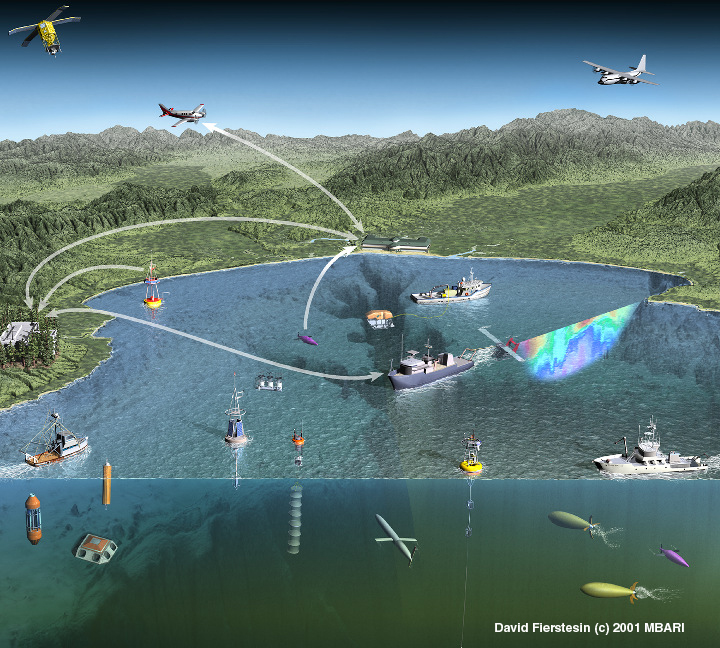
\includegraphics[width=3.3in]{MUSE_illus_pp.jpg}
\caption{Illustration of an oceanographic measurement campaign with multiple data collecting platforms.}
\label{fig:MUSE_illus_pp}
\end{figure}

This data access advantage does not exist for mobile platform \textit{in situ} measurement data stored in NetCDF files. Trajectory data is increasingly being collected by a variety of new platforms. These include all the measurements taken by vehicles such as ships, drifters, gliders, and AUVs (Fig.~\ref{fig:MUSE_illus_pp}). These data are structured in NetCDF files with one coordinate dimension: time. Even though the data are distributed through space the only index into the mini-database NetCDF file is time. There is no efficient way to retrieve specific spatial-temporal data directly from a trajectory NetCDF file. For example, if an application program needed to extract just the surface temperatures from a glider data file --- where the glider samples the water column in a sawtooth pattern from 0 to 500 meters depth --- it would have to read all of the data from the NetCDF file and then perform the extraction. This is a very inefficient way to access data; if the trajectory data were in a fully indexed relational database then applications can have efficient data access. STOQS is built upon a relational database and therefore provides optimal data access for data visualization and analysis purposes.

\begin{figure*}[hbp]
\centering
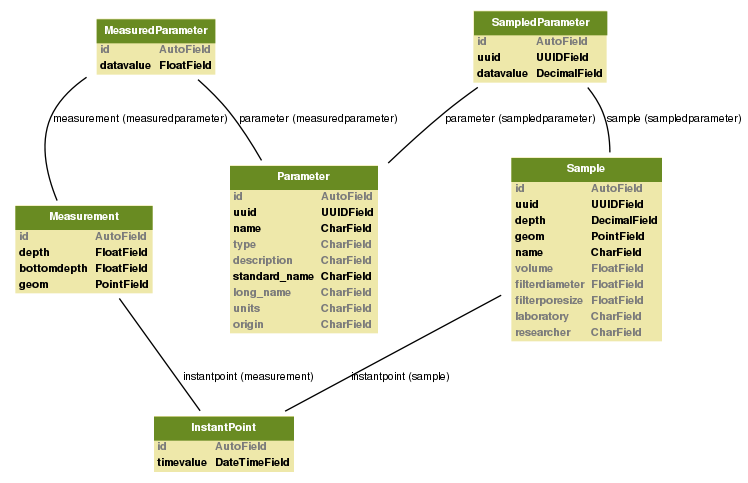
\includegraphics[scale=0.5]{stoqs_simple_model.png}
\caption{Key portion of STOQS database schema where spatial, temporal, and data values are stored. The database is normalized for efficient storage of data such that data are not repeated in any of the tables. Temporal and spatial data are stored separately in the InstantPoint and Measurement/Sample tables. For trajectory and timeseries data there is a one-to-one relationship for records in InstantPoint and Measurement/Sample. For timeseriesProfile and trajecotryProfile feature type data there are multiple Measurement/Sample records for each InstantPoint record. Parameter names are stored as records in the Parameter table allowing for new parameters without schema modification.}
\label{fig:stoqs_simple_model}
\end{figure*}

\subsection{Database Design}
A proper relational database design must consider many aspects of the scientific workflow: data ingestion, efficient storage, uniform search and access \cite{Bechini:2013:MSS:2425433.2425647}. The design of the STOQS database schema primarily focused on solving the problem of efficient access of \textbf{trajectory} data. However, care was taken to ensure that other discrete sampling geometry feature types \cite{DSG} that are common in oceanography would be supported by the schema.  The other feature type that have been common in MBARI's campaigns have been \textbf{timeseries} and \textbf{timeseriesProfile} which are produced by mooring deployments with instruments at a single depth and at multiple depths. 
A fourth feature type of \textbf{trajectoryProfile} is produced by profiling instruments aboard a moving platform; examples include shipboard ADCP and AUV measured mulibeam water column measurements. The STOQS schema can also store data of these kind of data.

Review of existing practices \cite{Wright} and \cite{MODB} informed the proper layout of the tables, fields and relationships.  The key portion of the STOQS data model which stores data is shown in Fig.~\ref{fig:stoqs_simple_model}. There are 29 other tables in the model which hold metatadata, statistics, and simplified representations which are used by the user interface to help with data visualization and access. The complete data model is available on the project's code repository \cite{STOQS}. 



\subsection{Architecture}

STOQS consists of a PostgreSQL/PostGIS database, Mapserver, and Python-Django running on a server and client-side technology (jQuery, OpenLayers, X3DOM, Twitter Bootstrap) running in a modern web browser (Fig.~\ref{fig:STOQSArch}) . The web application provides faceted search capabilities allowing a user to quickly drill into data of interest. Data selection can be constrained by spatial, temporal, and depth selections as well as by parameter values and platform names. The web application layer also provides a REST (Representational State Transfer) Application Programming Interface allowing tools such as Python, Matlab, and Google Earth to retrieve data directly from the database. The X3DOM JavaScript library provides interactive 3D views of the data in browsers that support WebGL.

\begin{figure}[htbp]
\centering
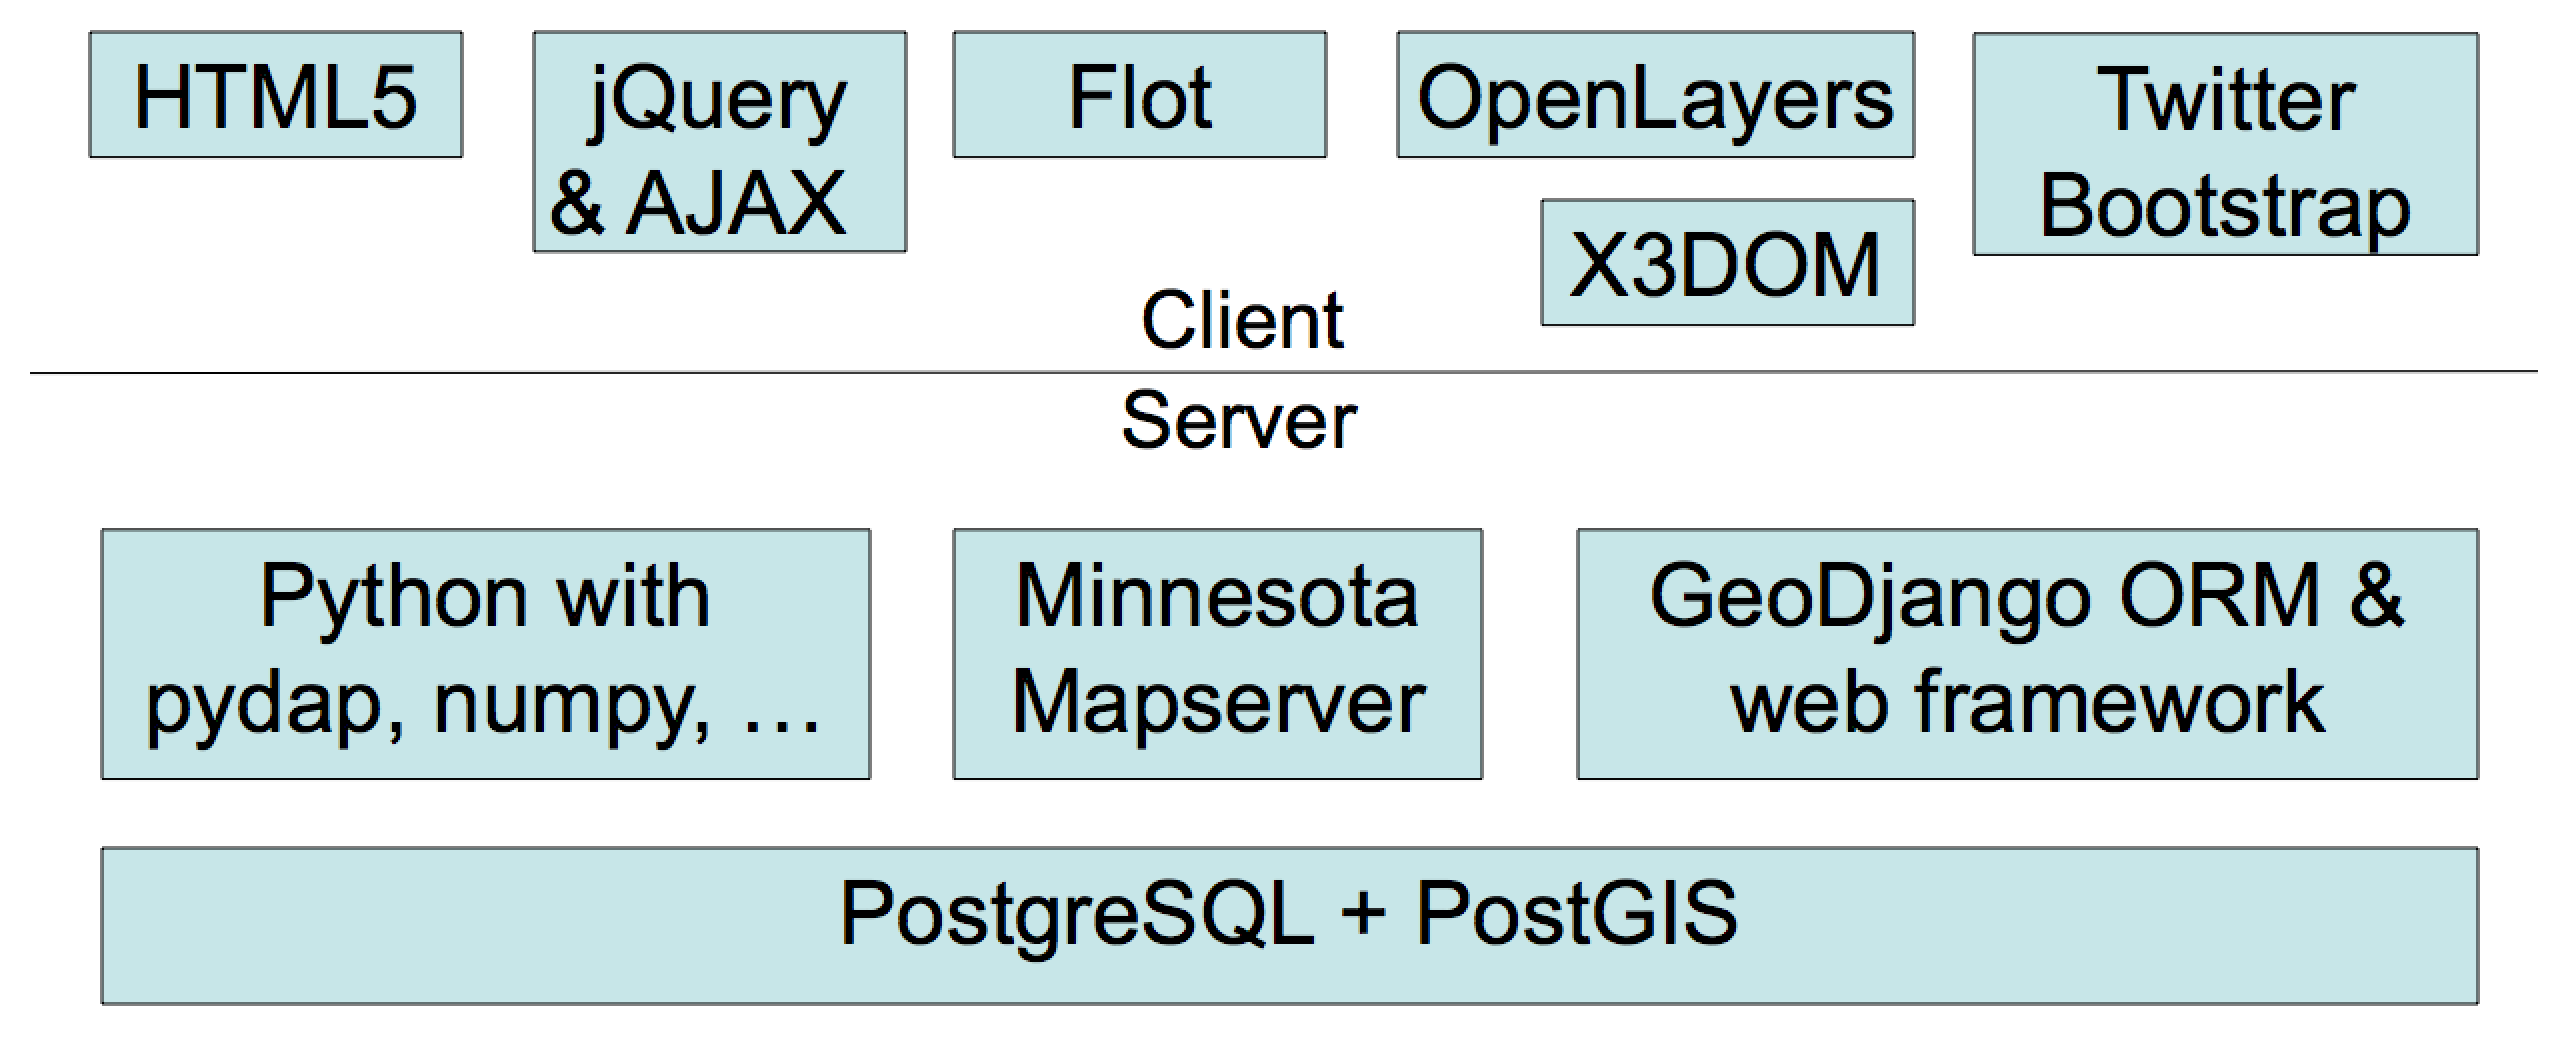
\includegraphics[width=3.3in]{stoqs_arch_simple.png}
\caption{STOQS integrates multiple open-source components.}
\label{fig:STOQSArch}
\end{figure}

\subsection{Metadata}

ISO 19135-2
Resource tables
friction-free data loads (free-form parameter name and CF standard\_name)


\section{Visualization}

\subsection{User Interface}

The STOQS User Interface displays a map of the vehicle tracks and a time series of depth profiles of the vehicles (Fig.~\ref{fig:STOQSscreencapture}). The bold blue letter text items are each sections that may be expanded revealing lists of items that may be selected for filtering, data selection, and plotting. If a platform is selected for filtering then only the information from that platform are shown in the other sections of the interface. Any selection initiates an instant update of the other items that may be selected. With this faceted search capability the user can quickly narrow a selection for data of interest. For instance in Fig.~\ref{fig:STOQSscreencapture} the platform "daphne"  and a time range of about a half a day have been selected. The interface is reactive to browser screen size and behaves appropriately when viewed on tablets and smart phones.

Within the web application data are retrieved directly from the database via XHR (XMLHttpRequest) requests delivering data in JSON (JavaScript Object Notation) data structures. Client-side JavaScript code then formats these data as needed for display in the web page. Any DOM (Document Model Object) element, such as buttons and checkbox labels can be updated with data from the database. In fact, requested data can update any DOM element, including elements in the 2D Temporal Flot plot an in  X3D scene graphs placed anywhere in the web page.

The overall design approach follows the so-called Shneiderman's mantra: "Overview first, zoom and filter, then details-on-demand" \cite{Whitney:2012:DIN:2597850}. This is in contrast to other data portal web sites which often present the user with empty text boxes in which unfamiliar users are at a loss on what to enter. The STOQS UI adheres to about 9 of the 12 elements of interactive dynamics described in \cite{Heer:2012:IDV:2133416.2146416}.

\begin{figure*}[htbp]
\centering
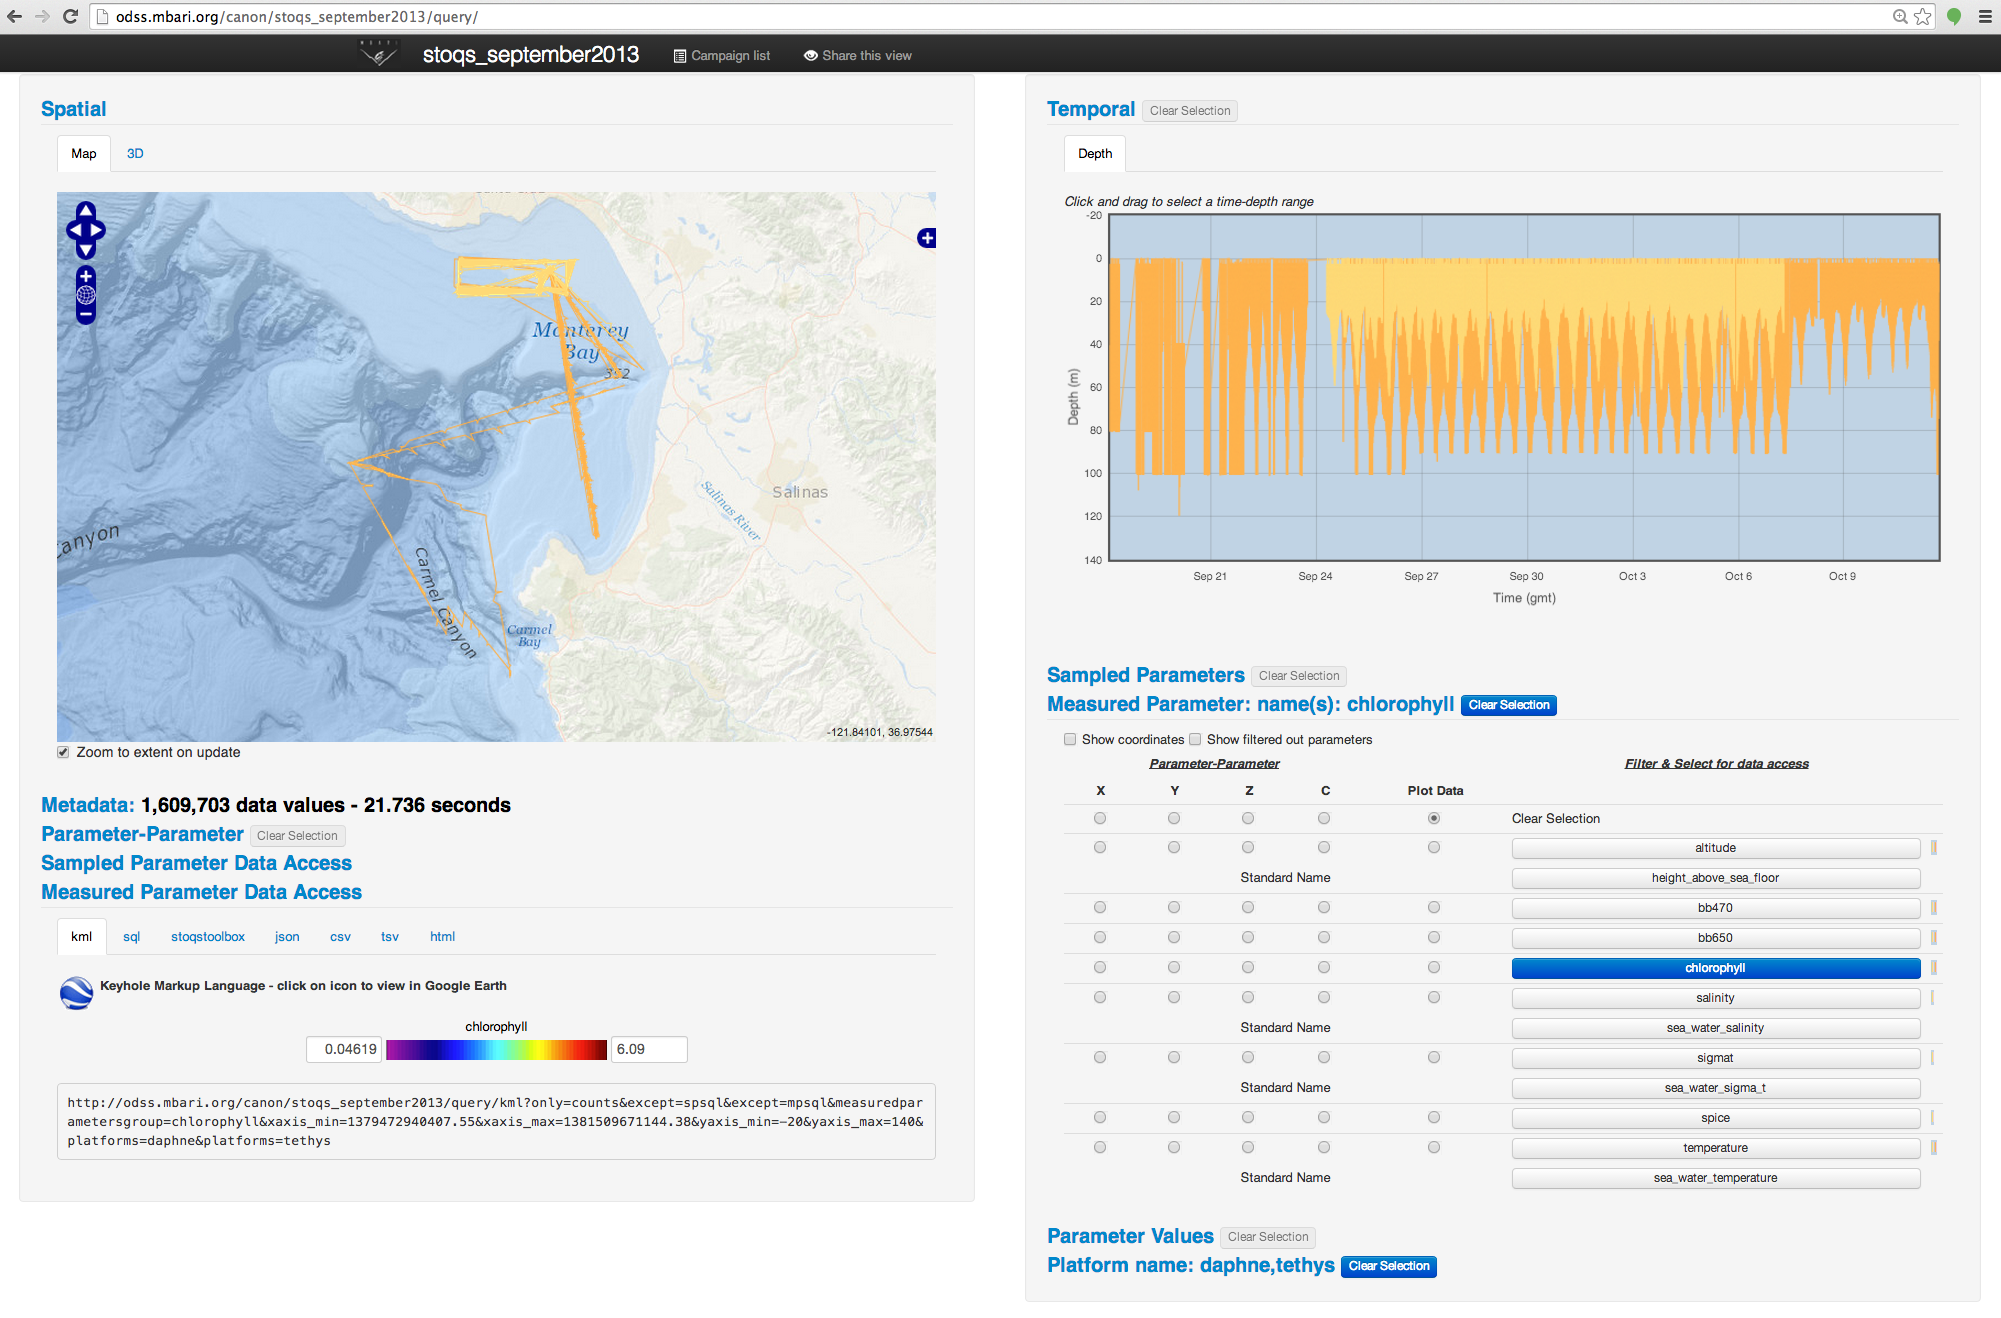
\includegraphics[width=6.6in]{STOQSscreencapture.png}
\caption{STOQS User Interface. Parameter chlorophyll is selected showing overview of when, where, and what platforms measured it.}
\label{fig:STOQSscreencapture}
\end{figure*}

\subsection{Spatial}

\subsubsection{2D}
The default spatial view in the STOQS UI is a 2D OpenLayers generated map. It shows simplified tracks of the vehicles over the selected basemap. The ESRI Ocean basemap is the default, but users can also select Open Street Maps and GEBCO \& NOAA Tiles, which is a local tile set for use aboard research vessels that do not have Internet connectivity. The track lines are generated on the server with a dynamically generated mapserver configuration file. Mapserver queries the database and builds image tiles which are then transmitted to the client using the OGC Web Map Service (WMS) protocol. As some campaigns contain dozens of tracks this approach performs better than individual transmission of vector data to the OpenLayers client code. Because WMS is a well established standard the server and client components - developed by different organizations - are able to work together using agreed upon request and response messages. If a user selects a Measured Parameter for plotting then a checkbox appears under the map for presentation of the sensor data as colored tracks on the map. These data are retrieved from the server with an XHR request and then delivered to OpenLayers as a vector layer in KML format. Performance degrades with more than about 300 points therefore server-side code subsamples large responses in order to maintain application responsiveness.

\subsubsection{3D}
Next to the Map tab in the Spatial section is a 3D tab. This 3D tab appears only for databases in which a terrain model has been loaded. A Python dictionary specifies the needed parameters for the STOQS UI to display a 3D terrain "basemap" (Fig.~\ref{fig:x3dTerrains}). Logic in the client code maps the position, orientation, and centerOfRotation values to the corresponding DOM elements in the scene graph. (The next section describes ways to construct X3D terrain models.)

\begin{figure}[htbp]
\centering
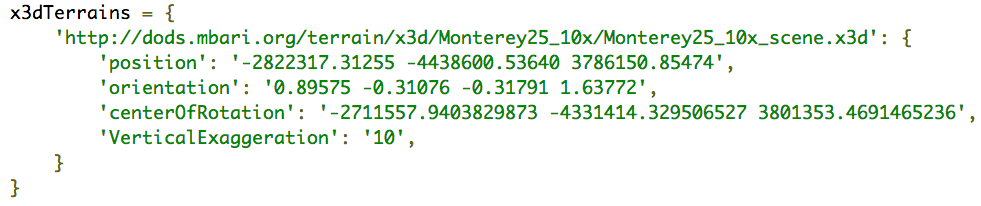
\includegraphics[width=3.3in]{x3dTerrains.png}
\caption{Dictionary of terrain information loaded into STOQS.}
\label{fig:x3dTerrains}
\end{figure}

Selected Measured Parameter data are delivered to the Spatial 3D display when a radio button in the Plot Data column is selected and the checkbox in the 3D panel is checked. The process for the update of the display is:

\begin{enumerate}
\item HTML contains X3D scene graph elements for the web page: Fig.~\ref{fig:Spatial3D_DOM}
\item Data are received by the browser from an XHR request in JSON format: Fig.~\ref{fig:JSONData}
\item jQuery JavaScript code takes the values from the JSON and writes them to the scene graph elements: Fig.~\ref{fig:jQueryDOMUpdateGeo}
\end{enumerate}

\begin{figure}[!htbp]
\centering
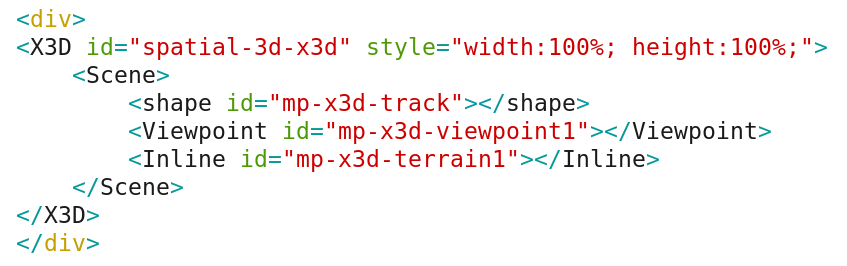
\includegraphics[width=3.3in]{Spatial3D_DOM.png}
\caption{X3D scene graph within the HTML before being updated.}
\label{fig:Spatial3D_DOM}
\end{figure}

\begin{figure}[!htbp]
\centering
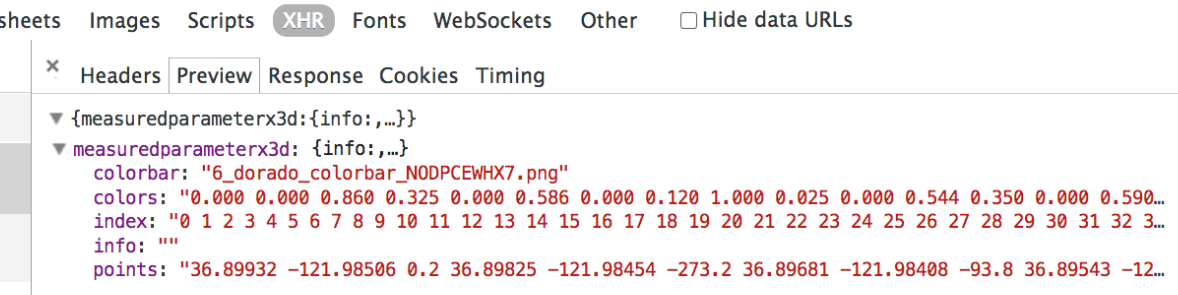
\includegraphics[width=3.3in]{JSONData.png}
\caption{Measured Parameter X3D data in JSON format returned by XHR request.}
\label{fig:JSONData}
\end{figure}

\begin{figure}[!htbp]
\centering
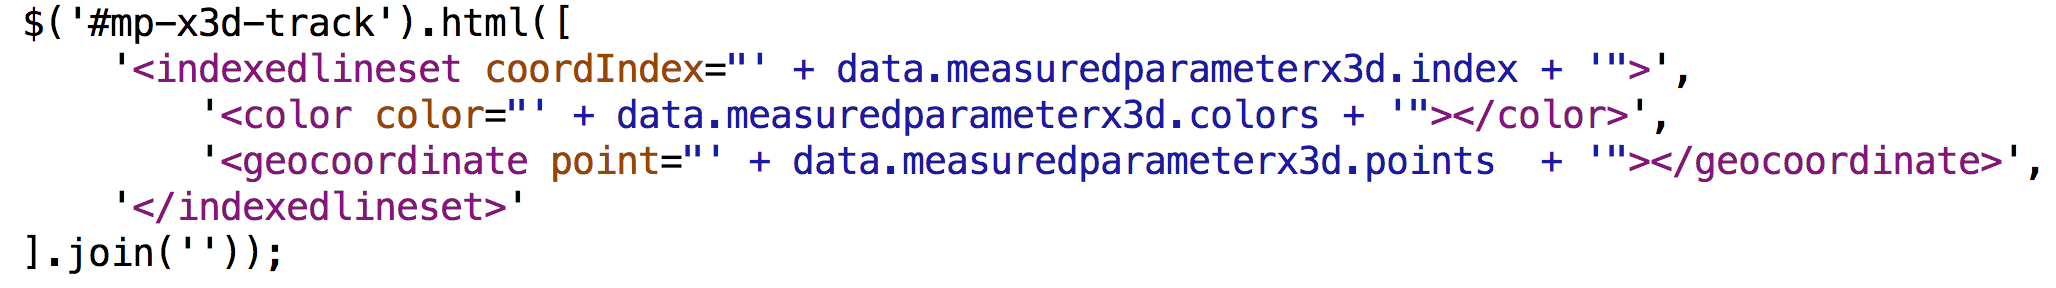
\includegraphics[width=3.3in]{jQueryDOMUpdateGeo.png}
\caption{JQuery JavaScript code that updates the X3D DOM elements.}
\label{fig:jQueryDOMUpdateGeo}
\end{figure}

Updates are triggered by any selections in the UI that would result in different data being displayed. An example would be selecting a smaller depth-time region in the Temporal section. Sensor data are represented in X3D as an IndexedLineSet built out of geocoordinate points, which is this case are latitude, longitude, and depth relative to the WGS84 ellipsoid, the default geosystem. X3D Geospatial performs the conversion of geodetic coordinates to geocentric coordinates which is the native coordinate system used by X3D Geospatial.

\subsection{Terrain Rendering}

As explored by \cite{yoo09} the Earth's terrain can be represented using GeoElevationGrid nodes. High resolution terrain can be structured in a nested quad-tree tile set using GeoLOD nodes. For representing data for the entire globe a multi-resolution approach such as this is a common. In fact, popular globe viewers such as Google Earth use this approach with sophisticated techniques to decide which tiles to load and unload depending on the users viewpoint and motion through the world. These techniques improve performance, are often proprietary, and can help distinguish a product within the marketplace. Similar techniques have not yet found their way into open source implementations of X3D Geospatial. However, small regions of the Earth can be represented in a single tile with enough horizontal resolution to be useful. MBARI's oceanographic campaigns are typically constrained to small geographic regions such as Monterey Bay and San Pedro Bay. For these regions a 50 meter gridded terrain model represented as a single GeoElevationGrid has less than a million vertices, which is effectively  rendered by today's 3D graphics hardware.

In 2013 \cite{Limper:2013:FDW:2466533.2466536} introduced Progressively Ordered Primitive (POP) buffers in X3DOM. Large POP geometry meshes (up to 1.5 million faces) are rendered with very good performance on today's computers with X3DOM. Advantages of representing bathymetric data in meshes is addressed by \cite{Becker:2005:NPN:1650409.1650513}. Meshes, in contrast to regular grids, are able to use fewer larger triangles for flat and smooth portions of terrain and more smaller triangles for the rugged portions of terrain. Besides providing more accurate representations of bathymetry meshes can also represent overhangs and caves, whereas GeoElevationGrids cannot. The workflow for creating the x3dterrain files using open source tools GMT \cite{GMT} and Meshlab \cite{Meshlab} is similar to that used in \cite{Silvestre}:

\begin{itemize}
\item Use GMT to create a point cloud in geocentric coordinates with 10x vertical exaggeration:
\begin{verbatim}
gmt grd2xyz Monterey25.grd \
  --D_FORMAT=%f | sed '/NaN/d' | \
  awk '{print $1, $2, 10 * $3}' | \ 
  mapproject -E --D_FORMAT=%f > \
  Monterey25_10x.asc
\end{verbatim}
\item Process interactively in Meslab:
\begin{itemize}
\item Load .asc file
\item Filter operations
\begin{itemize}
\item Point Sets - Compute normals for point sets
\item Surface Reconstruction: Poisson (Octree Depth: 12, Solver Divide: 10)
\item Remeshing, Simplification and Reconstruction - Quadric Edge Collapse Decimation:
\begin{itemize}
\item Target number of faces: 1,500,000
\item Preserve Normal
\item Preseve Topology
\item Optimal Position of Simplified Vertices
\item Planar Simplification
\item Post-simplification cleaning
\end{itemize}
\end{itemize}
\item Cleanup (with plenty of intermediate saves)
\item Filter - SmoothingÉ - Laplacian smooth (surface preserve)
\item Export mesh to .ply
\end{itemize}
\item Build X3D files with InstantReality aopt tool:
\begin{verbatim}
aopt -i Monterey25_10x-smooth.ply \
  -F Scene -b Monterey25_10x-opt.x3db
aopt -i Monterey25_10x-opt.x3db \
  -f PrimitiveSet:creaseAngle:4 -V \
  -K "binGeo/:ib" \
  -N Monterey25_10x.html
\end{verbatim}
\end{itemize}

These operations result in a static web page where the results can be tested for fidelity and performance. In order for the terrain model to be included in the STOQS UI the Scene elements are extracted from the HTML into a separate scene X3D file. This file and the associated binGeo files are what is referenced in Fig.~\ref{fig:x3dTerrains} for loading into STOQS. Fig.~\ref{fig:Monterey25_lrauvs} shows the terrain built with the above steps along with a the chlorophyll measurements of month-long deployments of 2 AUVs in Monterey Bay.

\begin{figure}[htbp]
\centering
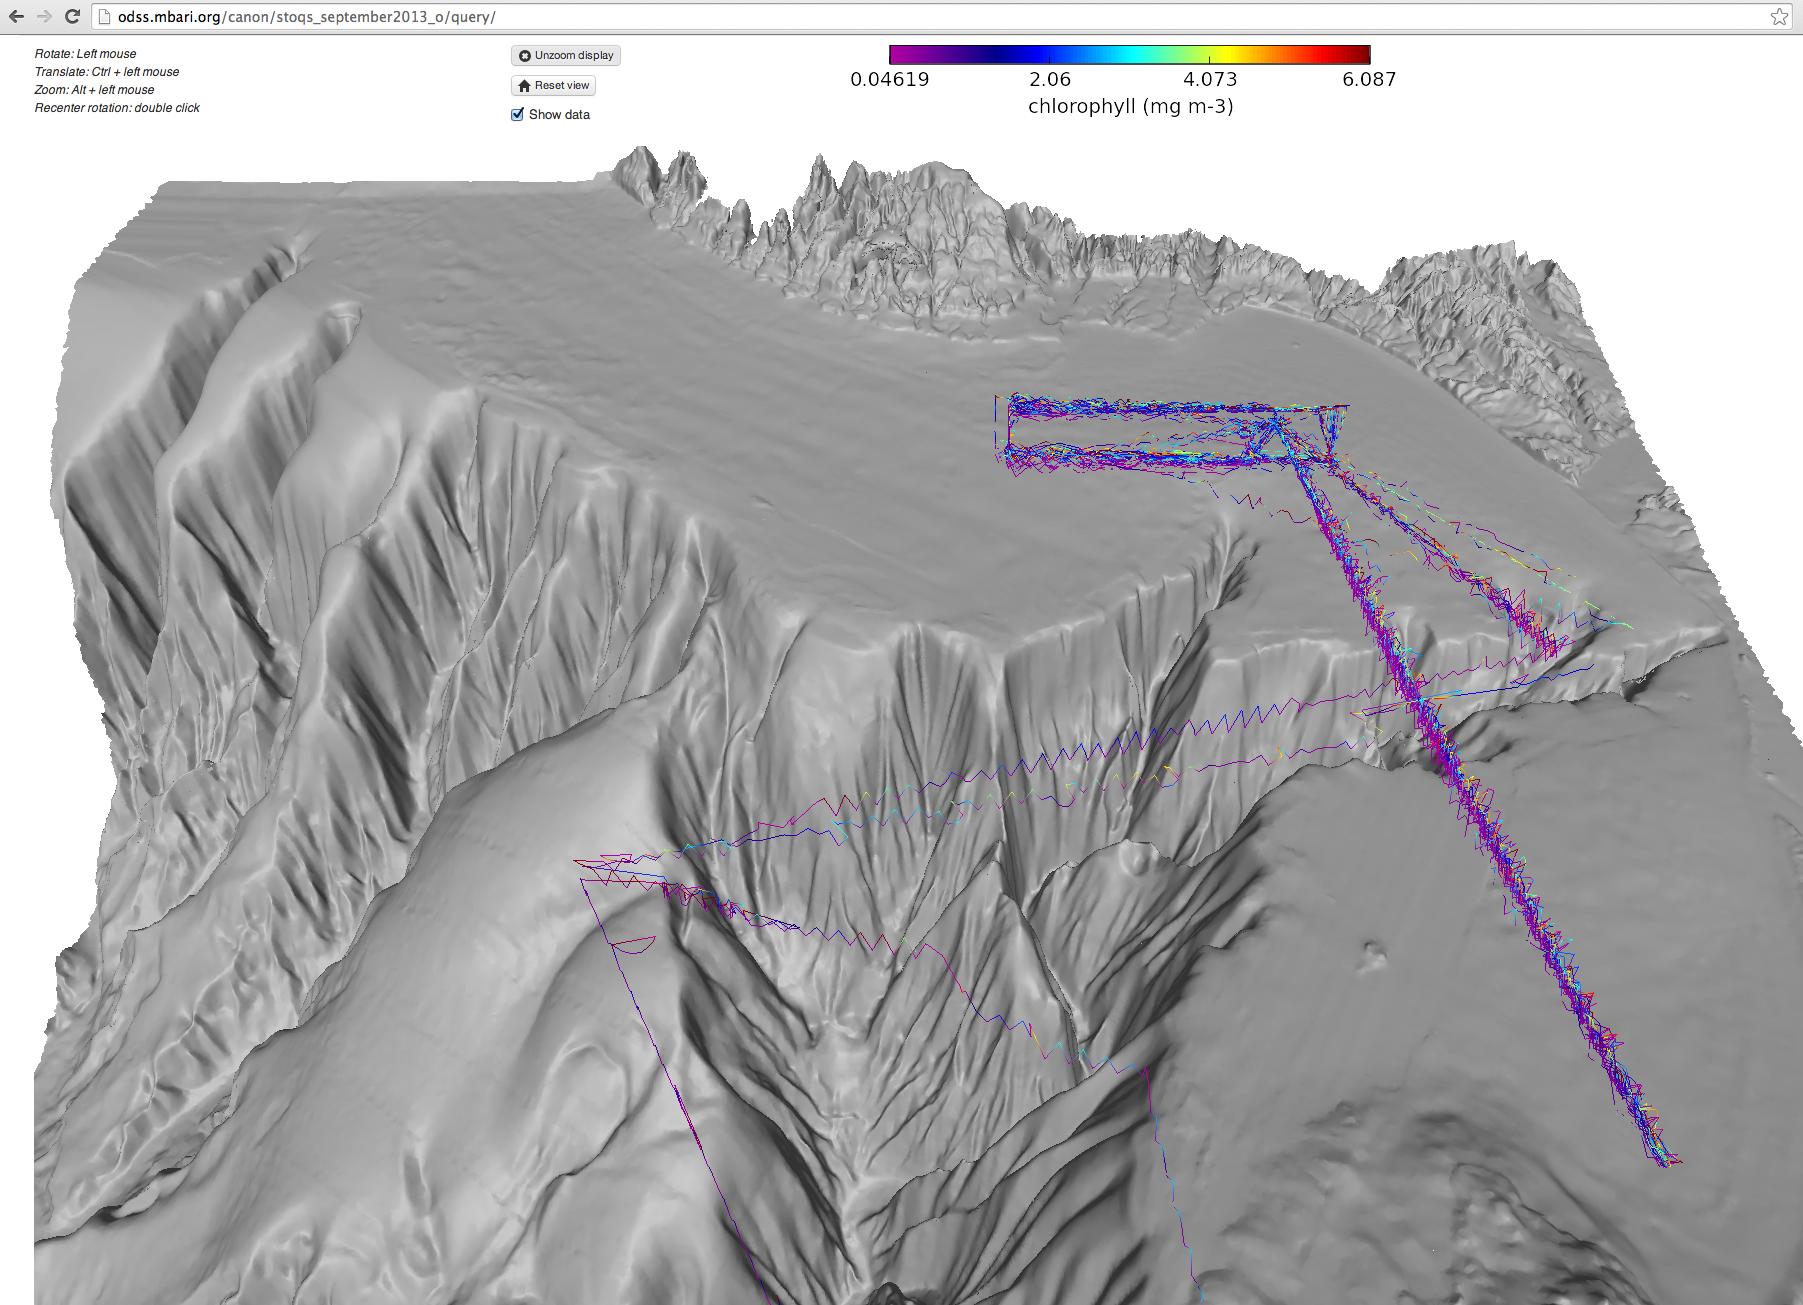
\includegraphics[width=3.3in]{Monterey25_lrauvs.png}
\caption{POP Geometry of 25m resolution Monterey Bay terrain with AUV measured chlorophyll data rendered by X3DOM in STOQS.}
\label{fig:Monterey25_lrauvs}
\end{figure}


\subsection{Temporal}

\subsubsection{Depth}
The default temporal display is the Depth tab where the vertical axis of the plot is depth. A depth versus time plot is appropriate for trajectory and timeseriesProfile data. The plotting space is interpreted as a depth section through time/distance. 

\subsubsection{Parameter}
The other display of temporal data is where the vertical axis is the value of parameter(s). This typical time series plot is appropriate for timeseries data that have been recorded by stationary platforms. 



\section{Using STOQS}

\subsection{Operation}

STOQS has been in use at MBARI for over 3 years to help manage and visualize data collected during upper water column measurement campaigns where scientific goals center on improving our understanding of biological processes. The data consist primarily of measurements collected by moving platforms. The platforms have accurate clocks, Global Positioning Sensors and underwater inertial navigation sensors, and one or more instruments that measure parameters such as temperature, salinity, oxygen, nitrate, chlorophyll fluorescence, optical backscatter, and particle sizes. Some platforms can also capture water samples for later laboratory analysis. A typical workflow for is:
\begin{enumerate}
\item Install the STOQS software on a Linux server
\item Vehicles conduct their missions, collecting data
\item Create NetCDF files of the instrument data
\item Construct and execute a STOQS load script
\item Access and visualize data using the STOQS UI
\end{enumerate}


\subsection{Loading Data}

In the fall of 2013, STOQS was used in the MBARI project CANON (Controlled, Agile, and Novel Observing Network) with the goal of 1) using STOQS during an ongoing campaign to assist in making optimal sampling decisions and 2) to train users how to load data.  The CANON project was well suited for this task as there were multiple platforms, multiple institutions, and the need for continual visual analysis during the campaign.  Over 3.4 million data points were loaded from 23 platforms, covering 126 measurements, over a 39 day period. 

The CANON project took place between September 9 to October 16 2013, in and around the Monterey Bay, CA with the following objectives: 
\begin{enumerate}
\item Identify and trace source water and seed populations for phytoplankton blooms in and out of Monterey Bay
\item Develop environmental indices that can be used to predict the location and timing of blooms with enough accuracy and speed to be used to trigger autonomous sampling
\item Develop an information processing and display system that can be used in real time to improve decision making and publication preparation in delayed mode
\end{enumerate}

To this end, a total of 27 platforms participated in the campaign: 4 ships, 3 AUVs, 8 gliders, 7 drifters, and 5 moorings.  Fig.~\ref{fig:ReikoFigure1} shows the location and tracks of the platforms.

\begin{figure}[htbp]
\centering
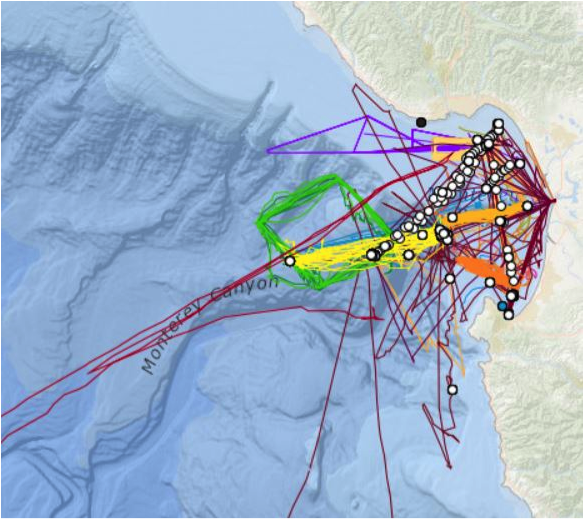
\includegraphics[width=3.3in]{ReikoFigure1.png}
\caption{STOQS map of the platforms used in the CANON Fall 2013 campaign in Monterey Bay, Central California.}
\label{fig:ReikoFigure1}
\end{figure}

Data from the platforms were received through a variety of portals and the data were in varying states of processing.  Some data were received hourly and other data on a daily basis.  The goal was to process the data as soon as possible and load it into STOQS for decision making.  The process was automated for all platforms, except for the ships, using cron scripts.  For STOQS loading, all data is required to be in NetCDF format.  Compliance with CF naming standards is needed to allow interaction between parameters from different platforms.  After raw data processing and NetCDF conversion, all data was loaded onto the CANON data repository, a THREDDS Server.  A Test STOQS installation was set up for the trainees where new load functions could be tested before loading to the production STOQS installation.   Fig.~\ref{fig:ReikoFigure2} illustrates the data flow.

\begin{figure}[htbp]
\centering
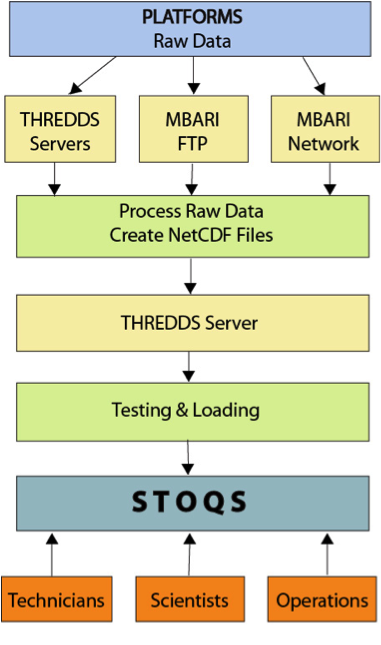
\includegraphics[width=2.0in]{ReikoFigure2.png}
\caption{Data flow.}
\label{fig:ReikoFigure2}
\end{figure}

Detailed load instructions can be found in the LOADING file at \cite{STOQS}. The MBARI CANON STOQS installation directory structure includes CANON subdirectories for load scripts and NetCDF conversion programs. Samples of python loading scripts can be found in the loaders/ project subdirectories. 

Loading data from a platform requires:

\begin{itemize}
\item CF-NetCDF Discrete Samping Geometry formatted data
\item Platform load functions
\item Platform load programs
\end{itemize}

Platform load functions are defined in the CANONLoader class in the python file loaders/\_\_init\_\_.py   A load function is created for each distinct platform, i.e. Dorado AUV, Tethys LRAUV, ESP mooring. The platform load script will call this function and pass the data location and data file parameters to begin loading data.  One may maintain a full and strided database; a strided data load is subsampled for quicker loading and exploration through the User Interface.

One of the requirements for using STOQS in the CANON campaign was to assist in decisions as the project was in progress. Quick exploration and visual analysis helped the team to assess the environmental conditions to guide AUVs, ships, and gliders.  The CANON project included platforms that were able to sample on a 24 hours basis: LRAUVs, moorings, drifters, and gliders. We automated loading by creating individual load scripts for platforms and using shell scripts scheduled to run using cron. 

In addition to individual loading of platforms, post campaign a master loading script was developed to load all the platform data at once.  This allows custom striding of data, the loading of quality controlled data, and a clean loading of all data sets.  In conclusion, the trainees were able to successfully load CANON campaign data.  Scientists were able to use the analytical tools to study biological dynamics and engineers were able to monitor platform and sensor performance.  



\subsection{Exploring Data}

\begin{figure}[htpb]
\centering
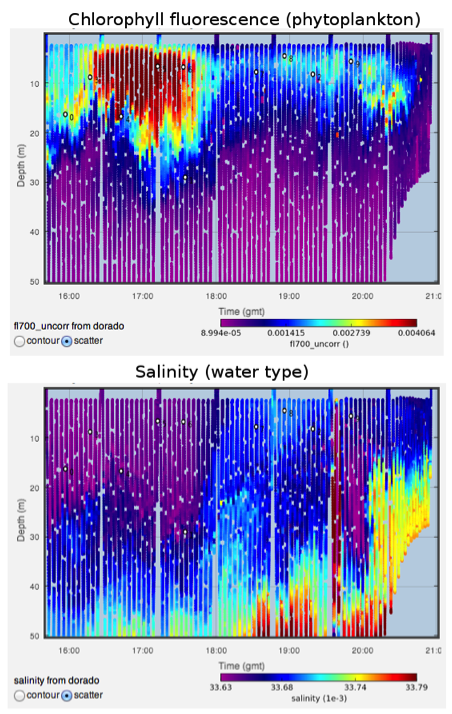
\includegraphics[width=3.3in]{JohnsFigureY.png}
\caption{Vertical sections of chlorophyll fluorescence (top) and salinity (bottom) for an AUV section from offshore (left) to onshore (right) across northern Monterey Bay on 16 September 2013.}
\label{fig:JohnsFigureY}
\end{figure}

\begin{figure}[htpb]
\centering
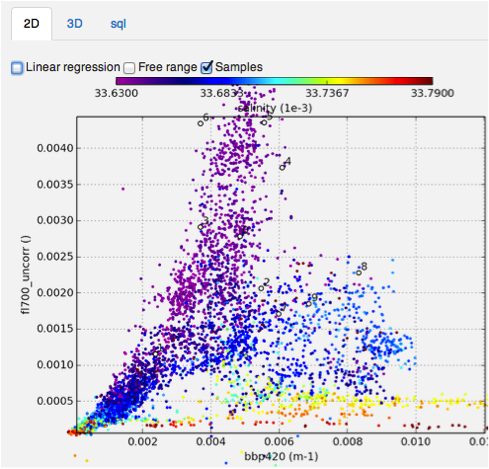
\includegraphics[width=3.3in]{JohnsFigureZ.png}
\caption{STOQS plot of the relationship between optical backscattering (x) and chlorophyll fluorescence (y), colored by salinity, for the AUV section shown in Fig.~\ref{fig:JohnsFigureY}.}
\label{fig:JohnsFigureZ}
\end{figure}

Property-property plotting revealed that the spatially separated phytoplankton populations exhibited different optical properties.  The offshore patch exhibited a higher ratio of chlorophyll fluorescence to optical backscattering (Fig.~\ref{fig:JohnsFigureZ}, high-chlorophyll points identified by the lowest salinity values).
Collecting high-resolution sections of multidisciplinary data, AUVs offer great potential for understanding marine ecology.  Yet the density and complexity of AUV data challenge efficient and effective exploration.  STOQS is facilitating exploration of AUV data from a variety of experiments.  Here we present an example exploration of AUV data in phytoplankton ecology research.

Occupying the core of the oceanic food web, phytoplankton (microscopic algae) are essential to ocean life, and their photosynthesis supplies about half of humanity’s oxygen needs.  While essential to earth’s biosphere, a small percentage of phytoplankton species can cause harm, for example by producing substances that are toxic to marine life and people.  Studying the ecology of harmful algal blooms (HABs) requires interdisciplinary research over a range of spatial and temporal scales, and AUVs provide excellent observations of phytoplankton patchiness and its relationship to environmental conditions at small to regional scales \cite{Scholin2000}.  Some AUVs can also acquire whole water samples autonomously targeted on phytoplankton patches, from which subsequent laboratory analyses can reveal phytoplankton identity and toxicity.  Supporting this research, STOQS integrates AUV data on the environment, optical characteristics of the phytoplankton, locations of sampling, and the data derived from shore-side laboratory analyses.

An experiment conducted during fall 2013 in Monterey Bay, California focused on HAB ecology, and it heavily employed AUVs (Fig.~\ref{fig:ReikoFigure1}).  

One of the primary HAB ecological questions concerns the source of seed populations for bloom events.  Seed populations for blooms may originate within our outside of Monterey Bay.  The first survey by a water-sampling AUV identified spatially separated phytoplankton populations within and outside the bay (Fig.~\ref{fig:JohnsFigureY}, top panel).  The population outside the bay had much higher chlorophyll fluorescence (left).  The separated phytoplankton populations occupied water of significantly different salinity (Fig.~\ref{fig:JohnsFigureY}, bottom panel), indicative of different ecological histories.


Water samples were acquired by the AUV from both phytoplankton populations (white circles in Fig.~\ref{fig:JohnsFigureY}).  Examination of these samples by microscopy revealed elevated abundances of a toxigenic species of diatom in the offshore patch.  This simple exploration thus represents the potential for developing optical proxies for phytoplankton ecotypes, as a tool for not only interpretation of data, but also refinement of autonomously targeted sampling by AUVs using optical data in real-time to control sample acquisition.

Beyond this simple illustration of AUV data exploration, the fusion of data from many other experiment platforms allows researchers to relate the AUV data to many other observations.



\section{Understanding Data}

\subsection{Labeling}
Today's oceanographic campaigns produce tens of millions of diverse measurements; this volume of data is too great for one to understand all of its information, even with an the effective user interface that STOQS provides.

The same database foundation that enables uniform data access for visualization purposes can be used for analytical purposes.

We are currently exploring ways to enhance data exploration and discovery using both supervised and unsupervised machine-learning methods.  These methods would produce tags that are stored in association tables that can be tied back to the actual data values.  

In the future, we envision these tags being further refined through expert validation, or as a feature to other processing, whether it is biological models or further machine learning models.  This is a challenging exploration and we are only in the beginning phases of this work. 

\subsection{Prediction}





% You must have at least 2 lines in the paragraph with the drop letter
% (should never be an issue)


% An example of a floating figure using the graphicx package.
% Note that \label must occur AFTER (or within) \caption.
% For figures, \caption should occur after the \includegraphics.
% Note that IEEEtran v1.7 and later has special internal code that
% is designed to preserve the operation of \label within \caption
% even when the captionsoff option is in effect. However, because
% of issues like this, it may be the safest practice to put all your
% \label just after \caption rather than within \caption{}.
%
% Reminder: the "draftcls" or "draftclsnofoot", not "draft", class
% option should be used if it is desired that the figures are to be
% displayed while in draft mode.
%
%\begin{figure}[!t]
%\centering
%\includegraphics[width=2.5in]{myfigure}
% where an .eps filename suffix will be assumed under latex, 
% and a .pdf suffix will be assumed for pdflatex; or what has been declared
% via \DeclareGraphicsExtensions.
%\caption{Simulation Results}
%\label{fig_sim}
%\end{figure}

% Note that IEEE typically puts floats only at the top, even when this
% results in a large percentage of a column being occupied by floats.


% An example of a double column floating figure using two subfigures.
% (The subfig.sty package must be loaded for this to work.)
% The subfigure \label commands are set within each subfloat command, the
% \label for the overall figure must come after \caption.
% \hfil must be used as a separator to get equal spacing.
% The subfigure.sty package works much the same way, except \subfigure is
% used instead of \subfloat.
%
%\begin{figure*}[!t]
%\centerline{\subfloat[Case I]\includegraphics[width=2.5in]{subfigcase1}%
%\label{fig_first_case}}
%\hfil
%\subfloat[Case II]{\includegraphics[width=2.5in]{subfigcase2}%
%\label{fig_second_case}}}
%\caption{Simulation results}
%\label{fig_sim}
%\end{figure*}
%
% Note that often IEEE papers with subfigures do not employ subfigure
% captions (using the optional argument to \subfloat), but instead will
% reference/describe all of them (a), (b), etc., within the main caption.


% An example of a floating table. Note that, for IEEE style tables, the 
% \caption command should come BEFORE the table. Table text will default to
% \footnotesize as IEEE normally uses this smaller font for tables.
% The \label must come after \caption as always.
%
%\begin{table}[!t]
%% increase table row spacing, adjust to taste
%\renewcommand{\arraystretch}{1.3}
% if using array.sty, it might be a good idea to tweak the value of
% \extrarowheight as needed to properly center the text within the cells
%\caption{An Example of a Table}
%\label{table_example}
%\centering
%% Some packages, such as MDW tools, offer better commands for making tables
%% than the plain LaTeX2e tabular which is used here.
%\begin{tabular}{|c||c|}
%\hline
%One & Two\\
%\hline
%Three & Four\\
%\hline
%\end{tabular}
%\end{table}


% Note that IEEE does not put floats in the very first column - or typically
% anywhere on the first page for that matter. Also, in-text middle ("here")
% positioning is not used. Most IEEE journals/conferences use top floats
% exclusively. Note that, LaTeX2e, unlike IEEE journals/conferences, places
% footnotes above bottom floats. This can be corrected via the \fnbelowfloat
% command of the stfloats package.



\section{Conclusion}
The STOQS platform has been successful ...





% conference papers do not normally have an appendix


% use section* for acknowledgement
\section*{Acknowledgements}

Appreciation is given to the numerous people involved in the deployment, recovery, operation and data handling for all of the platforms whose data are presented here. Development of STOQS is supported by the David and Lucile Packard Foundation at the Monterey Bay Aquarium Research Institute. It was inspired by the MOQuA tool originally developed by Mike Godin \cite{godin05}.




% trigger a \newpage just before the given reference
% number - used to balance the columns on the last page
% adjust value as needed - may need to be readjusted if
% the document is modified later
%\IEEEtriggeratref{8}
% The "triggered" command can be changed if desired:
%\IEEEtriggercmd{\enlargethispage{-5in}}

% references section

% can use a bibliography generated by BibTeX as a .bbl file
% BibTeX documentation can be easily obtained at:
% http://www.ctan.org/tex-archive/biblio/bibtex/contrib/doc/
% The IEEEtran BibTeX style support page is at:
% http://www.michaelshell.org/tex/ieeetran/bibtex/
\bibliographystyle{IEEEtran}
% argument is your BibTeX string definitions and bibliography database(s)
\bibliography{IEEEabrv,UsingSTOQS}
%
% <OR> manually copy in the resultant .bbl file
% set second argument of \begin to the number of references
% (used to reserve space for the reference number labels box)
%%\begin{thebibliography}{1}
%%
%%\bibitem{IEEEhowto:kopka}
%%H.~Kopka and P.~W. Daly, \emph{A Guide to \LaTeX}, 3rd~ed.\hskip 1em plus
%%  0.5em minus 0.4em\relax Harlow, England: Addison-Wesley, 1999.
%%\end{thebibliography}




% that's all folks
\end{document}


